\documentclass[../00_main.tex]{subfiles}

\begin{document}

\section{Educational Internship}

This section covers my educational internship at RS RAS. It covers NASA Remote
Sensing data, the netCDF data format, and libraries used to work with netCDF
files.

\subsection{NASA Remote Sensing Data}

NASA Earth Remote Sensing data is available via the Earth Science Data Systems 
(ESDS) Program (see \href{https://earthdata.nasa.gov/esds}{here}). The program 
covers the data acquisition, processing, and distribution to enable the 
widespread use of NASA mission data. The data is available for free and their
software is publicly available as Open Source Software 
\cite{esds-website}.\newline

Part of ESDS is the NASA Goddard Earth Sciences (GES) Data and Information 
Services Center (DISC) which provides data on atmospheric composition, water
and energy cycles, and climate variability \cite{gesdisc-about}. The GES DISC 
provides over 3.3 Petabytes of data \cite{gesdisc-main}, including the MERRA--2 
dataset. MERRA--2 (the Modern-Era Retrospective analysis for Research and 
Applications version 2) focuses on historical climate reanalysis using 
satellite data. The dataset I worked with (M2I3NPASM) contains data from 
January 1st, 1980 until October 1st, 2020 (at the time of writing). It covers 
the whole globe with measurements taken every 3 hours \cite{data-summary}. 
M2I3NPASM includes 14 measured variables in addition to latitude, longitude, 
time, and a pressure level. The measured variables include the surface 
pressure, specific humidity, eastward and northward wind, and temperature
\cite{data-readme}.\newline

The data is provided on the GES DISC website (see
\href{https://disc.gsfc.nasa.gov/datasets/M2I3NPASM_5.12.4/summary}{here}) and 
can be accessed from there. The website gives the option to download only a 
subset of the data by selecting a certain time range, latitude and longitude 
range, and a group of variables. This is advantageous because a full file for 
1 day is about 1.1 GB in size \cite{data-readme}.\newline

For my internship, I worked with a subset of the data that includes all
variables but is restricted to a latitude of 34\textdegree{}N to
48\textdegree{}N and longitude of 65\textdegree{}E to 83\textdegree{}E. This
geographical region is shown in \figref{map} below. It was created using
\href{https://www.openstreetmap.org/#map=5/43.787/69.565}{OpenStreetMap}. This
restricts the area to Kyrgyzstan and sections of all surrounding countries.
Additionally, the file size is reduced to a manageable 6 MB per file so that
a whole year of data only takes up 2.2 GB (in 365 files), the same space two
files of the complete data would take up.
\begin{figure}[H]
\center
    \fbox{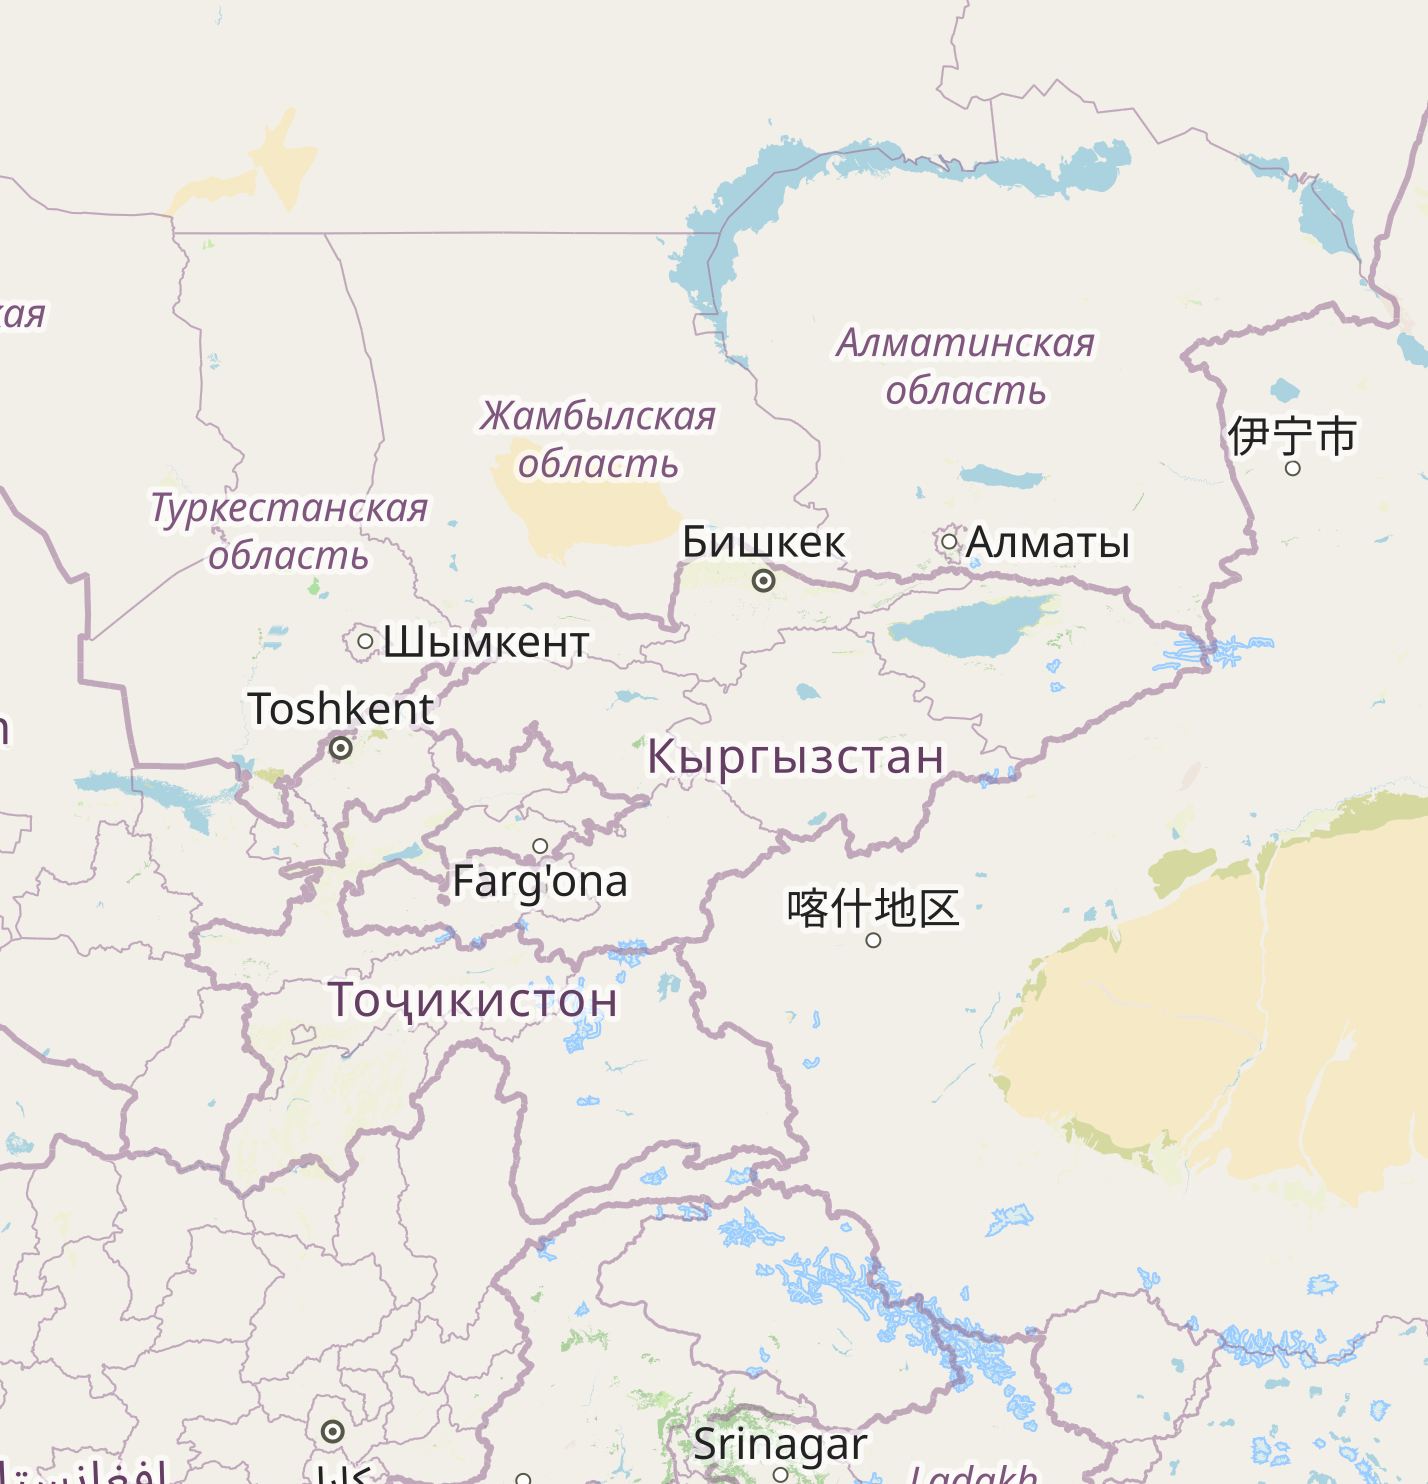
\includegraphics[width=0.9\textwidth]{../graphics/map}}
    \caption{OpenStreeMap view of the selected geographical region}
    \label{map}
\end{figure}

\subsection{The netCDF Data Format}

The M2I3NPASM data is provided in a file format called the Network Common Data 
Form (netCDF). NetCDF is made up of a data format and libraries that can read 
and write its data \cite{netcdf}. NetCDF is developed and maintained by 
Unidata, a community of research institutions, dedicated to sharing geoscience 
data and the tools to use and visualize it \cite{unidata}. Unidata is funded by 
the National Science Foundation, a US government agency that promotes and 
supports science and research \cite{nsf}. Unidata also maintains libraries 
(programming interfaces) for C, Java, and Fortran. Based on these, multiple 
other interfaces are available, including one for Python \cite{netcdf-facts}.
\newline

The netCDF data format is specifically designed to hold scientific data.
According to the Unidata website \cite{netcdf}, the netCDF data format has the 
following features:
\begin{itemize}
    \item \textbf{Self--Describing}. A netCDF file includes information about 
        the data it contains.
    \item \textbf{Portable}. A netCDF file can be accessed by computers with 
        different ways of storing integers, characters, and floating--point 
        numbers.
    \item \textbf{Scalable}. Small subsets of large datasets in various formats 
        maybe accessed efficiently through netCDF interfaces, even from remote 
        servers.
    \item \textbf{Appendable}. Data may be appended to a properly structured 
        netCDF file without copying the dataset or redefining its structure.
    \item \textbf{Sharable}. One writer and multiple readers may simultaneously 
        access the same netCDF file.
    \item \textbf{Archivable}. Access to all earlier forms of netCDF data will 
        be supported by current and future versions of the software.
\end{itemize}
The NASA M2I3NPASM data is available in "classic" netCDF--4 format, meaning that
it is backwards compatible. These files have 4 dimensions \cite{merra2-files}
(or 3, if the data does not depend on pressure):
\begin{enumerate}
    \item longitude in degrees east (meaning west is represented as negative),
    \item latitude in degrees north (making south negative),
    \item pressure in hPa,
    \item time in minutes since the first time point in a file.
\end{enumerate}
To be self--describing, the NASA M2I3NPASM netCDF files contain information
about, among others, the institution that created the file, the date and time 
of the beginning and end of the dataset, and the minimum and maximum latitude 
and longitude values \cite{merra2-files}. The files furthermore contain 
metadata for each of the measured variables \cite{merra2-files}. The most 
important of these are the fill values that identify missing data, the long 
name -- a full version of the short variable name abbreviation -- and the units 
of the variable.

\subsection{NetCDF Libraries}

Because I am working with the Python programming language for my internship
I require a netCDF library that works in that programming language. Unidata
provides an interface between the netCDF library for the C programming language
and Python. This interface is called netCDF4. It has most of the features of
the C library and enables the creation and reading of netCDF files using
Python \cite{netcdf4}. I use this interface to work with the netCDF files 
downloaded from GES DISC.

\end{document}
